%=====================
%  MATHEMATICS
%=====================

\begin{figure*}[!tb]
	\begin{subfigure}[t]{0.5\textwidth}
		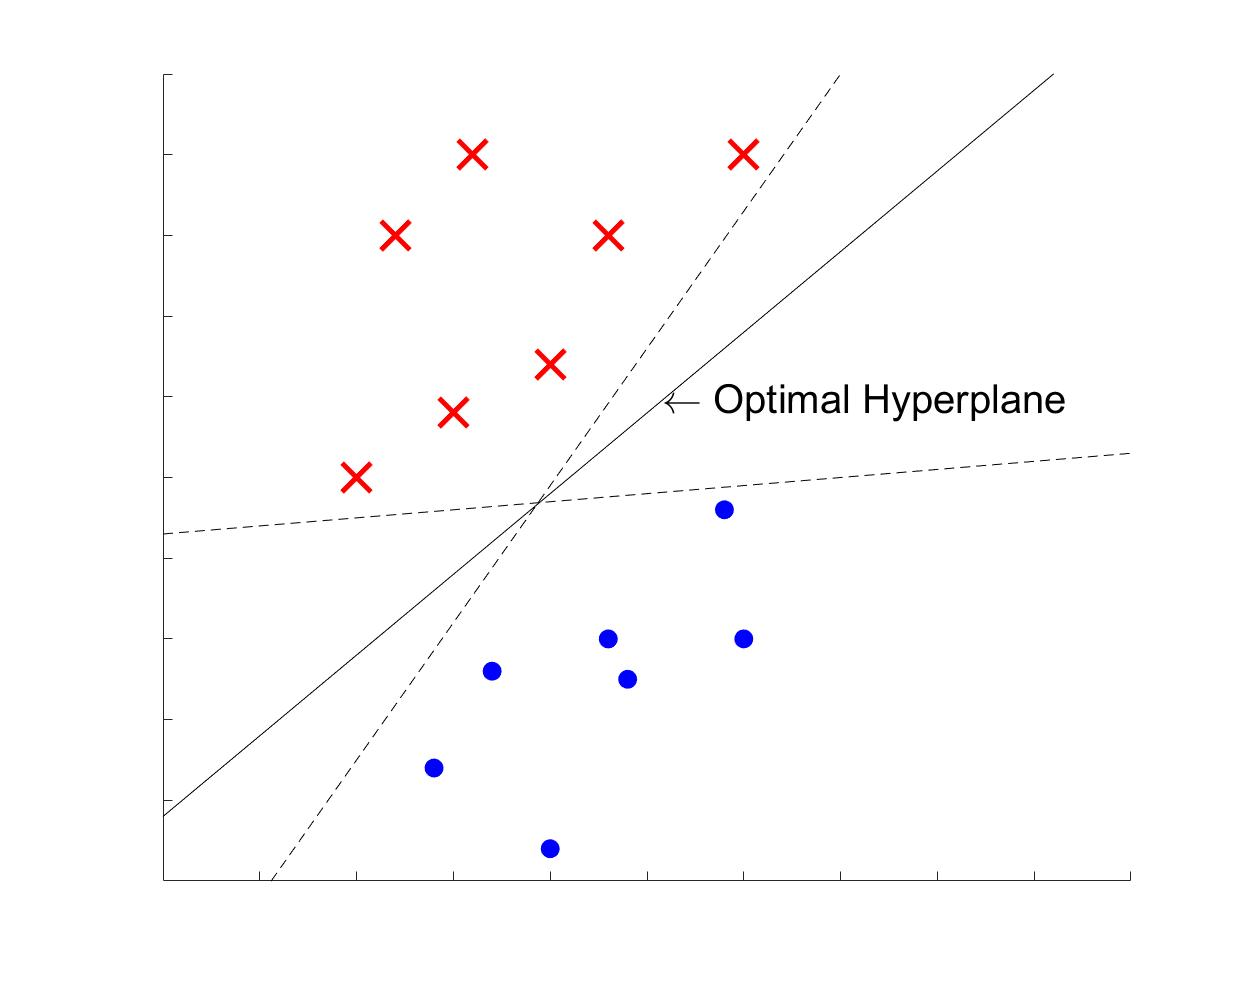
\includegraphics[width=7cm, height=7cm]{SVM_fig}
		\caption{Finding the optimal hyperplane}
		\centering
		\label{fig:SVM_fig_a}
	\end{subfigure}%
	~
	\begin{subfigure}[t]{0.5\textwidth}
		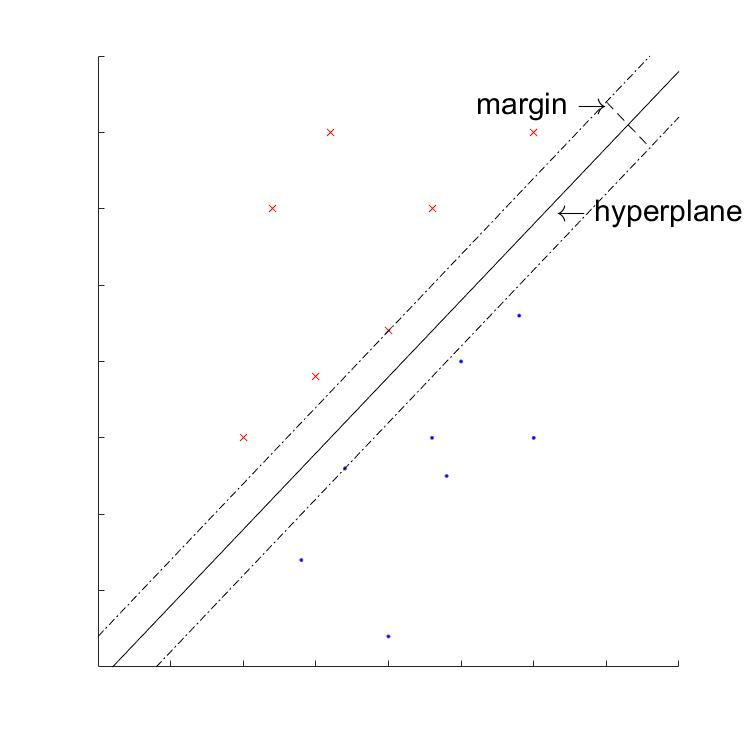
\includegraphics[width=7cm, 			height=7cm]{SVM_fig2}
		\caption{The optimal hyperplane}
		\centering
		\label{fig:SVM_fig_b}
	\end{subfigure}%
	
	\caption{Figure \ref{fig:SVM_fig_a} shows $3$ different separating hyperplanes, however only one separates the data most naturally. This is called the optimal hyperplane. Figure \ref{fig:SVM_fig_b} shows the optimal hyperplane, the margin planes, and the support vectors.}
	\label{fig:SVM_fig}
\end{figure*}

The concept of Support Vector Machines is very simple. It is a classifier that classifies data into two different classes by constructing a hyperplane that separates the two different classes. Figure \ref{fig:SVM_fig} illustrates a simple example.

Suppose we have training data:
\begin{gather}
(\vec{x_1}, y_1),  (\vec{x_2}, y_2), \dots, (\vec{x_m}, y_m) \nonumber\\
\vec{x_i} \in \mathbb{R}^{n} \quad\text{and}\quad y_i \in \{1, -1\} \nonumber
\end{gather}

where $1$ and $-1$ represent the two classes. We have chosen $ y_i \in \{1, -1\}$ because it makes the math simpler and cleaner, as will see. Now, suppose that the training data can be separated by the hyperplane\footnote{An important assumption we make is that the training data are linearly separable. We will later see how we can satisfy this assumption}:
\begin{equation}
\vec{w}\cdot\vec{x} + b = 0 \label{eq:optimal-plane}
\end{equation}

We construct this hyperplane such that:
\begin{gather}
\vec{w}\cdot\vec{x_i} + b \geq 1 \text{ if $y_i = 1$,} \label{eq:class-1} \\
\vec{w}\cdot\vec{x_i} + b \leq -1 \text{ if $y_i = -1$} \label{eq:notclass-1} 
\end{gather}

Once again, choice of $1$ and $-1$ for our margins are arbitrary. Now, notice that we have also constructed two planes that are parallel to our separating plane (\ref{eq:optimal-plane}). These planes form the margin for their respective classes.
\begin{gather}
\vec{w}\cdot\vec{x} + b = 1 \label{eq:margin-class-1} \\
\vec{w}\cdot\vec{x} + b = -1 \label{eq:margin-notclass-1}
\end{gather}

Generally, there are infinitely many hyperplanes that are able to separate the data. To find the \textit{best} hyperplane (the optimal hyperplane) that separates the two classes, we want to maximize the distance between the two margin hyperplanes. This supports our intuition that the \textit{best} separating plane should be as far away from both the classes as possible. See figure \ref{fig:SVM_fig_a} to understand why this supports our intuition.

The distance between the margin hyperplanes is given by\footnote{See Appendix \ref{appendix:distance} for proof}:
\begin{equation}
d = \frac{2}{\norm{\vec{w}}} \label{eq:margin-dist}
\end{equation}

The $2$ in the numerator is consequence of our choice that $y_i \in \{1, -1\}$. We want to maximize the distance, and maximizing the distance can be thought of as minimizing $\frac{\norm{\vec{w}}}{2}$. And minimizing $\frac{\norm{\vec{w}}}{2}$ is the same as minimizing $\frac{\norm{\vec{w}}^2}{2}$. So now, we have our optimization problem:
\begin{gather}
	\min_{\vec{w}, b} \frac{1}{2}\norm{w}^2 \nonumber\\
	\text{s.t. }
	\begin{cases}
	\begin{aligned}
		\vec{w}\cdot\vec{x_i} + b \geq 1 \text{ if $y_i = 1$} \nonumber\\
		\vec{w}\cdot\vec{x_i} + b \leq -1 \text{ if $y_i = 1$} \nonumber
	\end{aligned}
	\end{cases}
\end{gather}

This turns out to be a Quadratic Programming Problem, and beyond the scope of this report\footnote{See Appendix \ref{appendix:optimization} for a discussion of this optimization problem in detail}. But, it turns out that our choice of $1$ and $-1$ for the margins in equations (\ref{eq:margin-class-1}-\ref{eq:margin-notclass-1}) help make this problem is optimal i.e., it can be optimized subject to the constraints we have.

One of the constraints of the optimization problem that can be derived is \footnote{See Appendix \ref{appendix:optimization} for details}:
\begin{equation}
\vec{w} = \sum_{i = 1}^{m}\alpha_{i}y_{i}\vec{x_i} \label{eq:w-and-x}
\end{equation}

where $\alpha_{i}$ are the Lagrange multipliers. From this, we can deduce that the vector orthogonal to the optimal hyperplane is a linear combination of the input vectors i.e.,
\begin{gather}
	\vec{w} \in \text{span}(\vec{x_1}, \vec{x_2}, \dots, \vec{x_n}) \label{eq:normal-inputs} \\
	\vec{w} \in \text{rng}(X); \quad X = (\vec{x_1} \ \vec{x_2} \ \dots \ \vec{x_n})
\end{gather}

We do not know anything about the independence of $\{\vec{x_1}, \vec{x_2}, \dots, \vec{x_n}\}$. So, we cannot say anything about the basis and dimension of $X$. Also, with equation (\ref{eq:w-and-x}), we can now rewrite our optimal hyperplane as:
\begin{align}
	\vec{w}\cdot\vec{x} + b = \Big(\sum_{i = 1}^{m}\alpha_{i}y_{i}\vec{x_i}\Big)^{\text{T}}\vec{x} + b \nonumber \\
= \sum_{i = 1}^{m}\alpha_{i}y_{i}\langle\vec{x_i}, \vec{x}\rangle + b \label{eq:new-plane}
\end{align}

Now, let us turn our attention back to the margin hyperplanes. Notice that these hyperplanes are defined by the vectors that are the closest to the optimal hyperplane. And these vectors determine our margin, and thus our optimization problem. Hence, these vectors are called \textbf{Support Vectors} and thus this technique is called \textit{Support Vector Machines}. Figure \ref{fig:SVM_fig_b} shows the support vectors for our simple example.

\begin{figure*}[!tb]
	\centering
	\begin{subfigure}[t]{0.5\textwidth}
		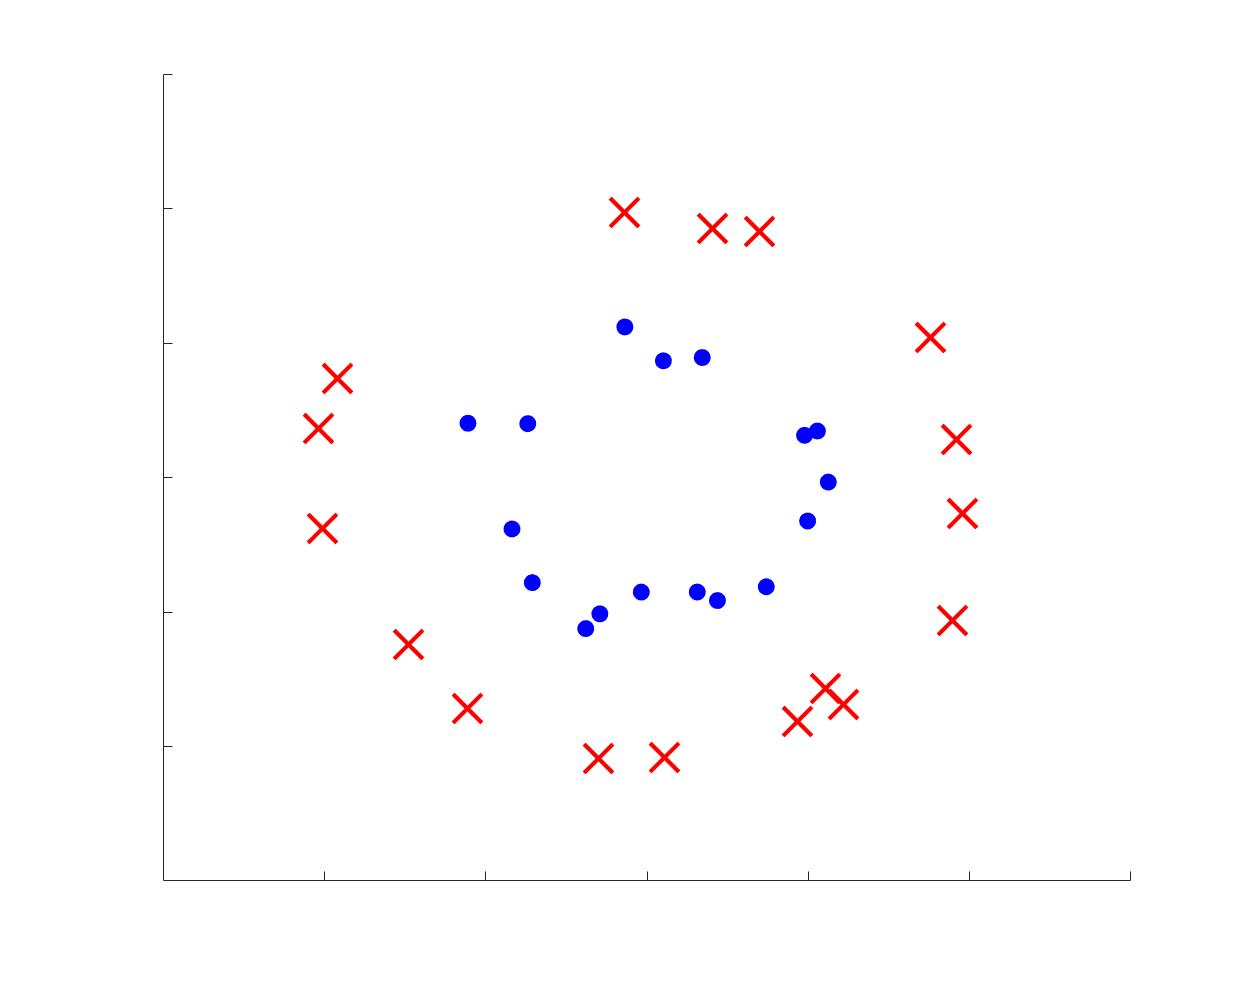
\includegraphics[width=7cm, height=7cm]{pre-transformation}
		\caption{Initial raw data}
		\centering
		\label{fig:pre-trans}
	\end{subfigure}%
	~
	\begin{subfigure}[t]{0.5\textwidth}
		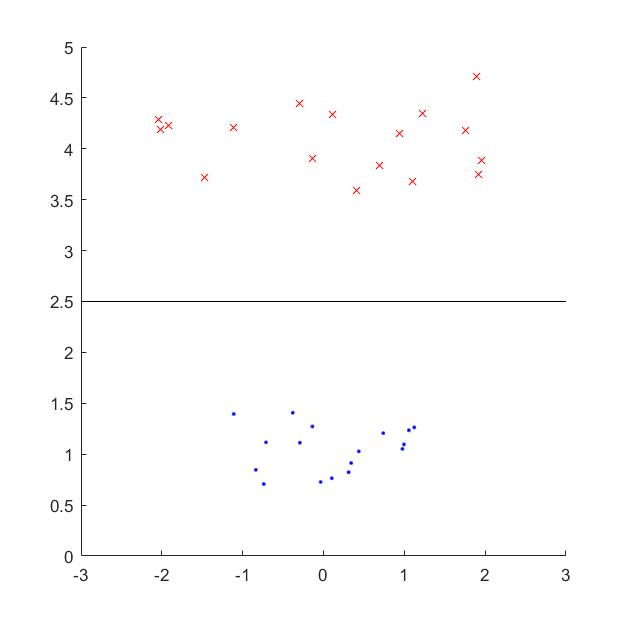
\includegraphics[width=7cm, 			height=7cm]{post-transform}
		\caption{Data transformed with a kernel}
		\centering
		\label{fig:post-trans}
	\end{subfigure}%
	
	\caption{Initially, the data, (\ref{fig:pre-trans}), is not linearly separable i.e., cannot be separated by a hyperplane. After applying a kernel transform, our transformed data, (\ref{fig:post-trans}), becomes linearly separable. Now, we can use a Support Vector Machine to classify the data.}	
	\label{fig:kernel}
\end{figure*}

Going back to our assumption that the data we have are linearly separable, we know that this assumption is not always valid. So, we can use something called a \textbf{Kernel}. This technique employs a transformation on the input data to transform the data into a different space, one that is now linearly separable.

Figure \ref{fig:kernel} illustrates a simple example where we use a kernel transform to be able to linearly separate our data. A kernel can be thought of as a transformation function applied to the data. A kernel function is usually nonlinear. Using a linear transformation as the kernel would be futile because, the representation matrix of the linear transform, $A$, would get absorbed by the normal vector of the hyperplane, $\vec{w}$, leaving us with the raw untransformed data again as seen below:
\begin{gather}
\begin{aligned}
	\vec{x^{'}} = \mathcal{L}[\vec{x}] = A\vec{x} \nonumber\\
	\vec{w}\cdot\vec{x^{'}} + b = 0 \nonumber\\
	\vec{w}\cdot (A\vec{x}) + b = 0 \nonumber\\
	(\vec{w}A)\cdot\vec{x} + b = 0 \nonumber\\
	\vec{w^{'}}\cdot\vec{x} + b = 0
\end{aligned}
\end{gather}

We can also think of kernels as replacing the inner products in equation (\ref{eq:new-plane}) with different feature mappings. For instance, if we have a feature mapping $\phi(\vec{x})$, we can replace the inner product with the corresponding Kernel to be:
\begin{equation*}
K(\vec{x}, \vec{y}) = \phi(\vec{x})^{\text{T}}\phi(\vec{y})
\end{equation*}

For instance, we can define a new polynomial kernel of degree $n$ as:
\begin{equation*}
K(\vec{x}, \vec{y}) = (\vec{x}^{\text{T}}\vec{y} + c)^n
\end{equation*}

where $c$ is a parameter that controls the relative weighting of $\vec{x}$ and $\vec{y}$. It turns out that there is a feature mapping $\phi$ that corresponds to this kernel function. More generally, we can use $K$ as a kernel function only if it corresponds to a feature mapping $\phi$ i.e., $K(\vec{x}, \vec{y}) = \phi(\vec{x})^{\text{T}}\phi(\vec{y})$ for all $\vec{x}, \vec{y}$.

Suppose that $K$ is a valid kernel corresponding to a feature mapping $\phi$. Then, consider a set of $n$ vectors $\{\vec{x_1}, \vec{x_2}, \dots, \vec{x_n}\}$. Now, we can define a matrix, called Kernel Matrix $K$, whose $(i,j)^{th}$ entry is given by $K_{ij} = K(\vec{x_i}, \vec{x_j})$. Note that we have overloaded $K$ with both the kernel function and the Kernel matrix.
If $K$ is a valid Kernel, then $K_{ji} = K(\vec{x_j}, \vec{x_i}) = \phi(\vec{x_j})^{\text{T}}\phi(\vec{x_i}) = \phi(\vec{x_i})^{\text{T}}\phi(\vec{x_j}) = K(\vec{x_i}, \vec{x_j}) = K_{ij}$. Thus, $K$ is symmetric. Let $\phi_k(\vec{x})$ denote the $k$-th coordinate of the $\phi(\vec{x})$ vector. And, let $\vec{z}$ be a vector in $\mathbb{R}^n$.
\begin{align}
	\vec{z}K\vec{z} &= \sum_{i}\sum_{j} z_{i}K_{ij}z_{j} \nonumber \\
&= \sum_{i}\sum_{j} z_{i}K(\phi(\vec{x_i}), \phi(\vec{x_j}))z_{j} \nonumber \\
&= \sum_{i}\sum_{j} z_{i}\sum_{k} K(\phi_k(\vec{x_i}), \phi_k(\vec{x_j}))z_{j} \nonumber \\
&= \sum_{k}\sum_{i}\sum_{j} z_{i}K(\phi_k(\vec{x_i}), \phi_k(\vec{x_j}))z_{j} \nonumber \\
&= \sum_{k} \Bigg(\sum_{i} z_i\phi_{k}(\vec{x})\Bigg)^2 \nonumber \\
&\geq 0 \label{eq:kernel-psd}
\end{align}

From equation (\ref{eq:kernel-psd}), we know that the Kernel matrix is positive semi-definite ($K \geq 0$). Hence, if $K$ is a valid kernel (i.e., corresponds to a feature mapping $\phi$), then the corresponding Kernel matrix $K \in \mathbb{R}^{n\times n}$ is symmetric positive definite. More generally, it turns out that this not just a necessary, but also a sufficient, condition for $K$ to be a valid kernel.

We must take care when using a kernel transformation. Using the wrong transformation can worsen our results. For instance, if we initially had data that was linearly separable and transformed it with, say, the polar transformation, then our new feature space (transformed data) is no longer linearly separable, decreasing the accuracy of our classifier.